% Chapter 2

\chapter{Deep Learning theory and Related Derivated} % Main chapter title

\label{Chapter2} % For referencing the chapter elsewhere, use \ref{Chapter1} 

\setlength{\parindent}{0pt}
%----------------------------------------------------------------------------------------

\section{Recurrent Neural networks}

Artificial neural networks usually only fetch and process one input individually, and the previous input has nothing to do with the next input. However, some tasks need to handle sequence information better, which means the previous input is related to the subsequent input. In this kind of problem, former researchers Graves and Alex(2009) designed the recurrent neural network (RNN), which is a class of artificial neural networks where connections between nodes form a directed graph along a temporal sequence. This allows it to exhibit temporal dynamic behavior. Derived from feedforward neural networks, RNNs can use their internal state (memory) to process variable-length sequences of inputs.

Sepp Hochreiter and Jürgen Schmidhuber (1997) post the practical method under the concept of RNN, that is, Long short-term memory (LSTM) architecture, with both feedforward neural networks and feedback connections.  This makes them applicable to tasks such as unsegmented, connected handwriting recognition, or speech recognition.

\section{Convolutional Neural Networks and TCN}

Convolutional Neural Networks(CNNs) were originally used on two-dimensional and three-dimensional images, but they are also suitable for one-dimensional data such as univariate time series. Shaojie Bai, J. Zico Kolter, and Vladlen Koltun(2018) designed the architecture temporal convolutional network(TCN) and ran it into image, sound, and text level tasks. This work inspired that convolutional networks could reach the same even better results as other sequence models. Alberto(2019) experimented with TCN and other sequence models in smart grids situations, also found that convolutional networks are significantly useful in time series tasks. However, Seq2Seq methods still hold the best performance place.

\subsection{The origin of TCN}
The Temporal Convolutional Networks (TCNs) was first proposed by the work of Lea et al. (2016) for video-based action segmentation. The two steps of this conventional process include: firstly, computing of low-level features using (usually) CNN that encode spatial-temporal information and secondly, input these low-level features into a classifier that captures high-level temporal information using (usually) RNN. The main disadvantage of such an approach is that it requires two separate models. TCN provides a unified approach to capture all two levels of information hierarchically.

\subsubsection{Encoder-Decoder TCN} The encoder-decoder framework is presented in below, where further information regarding the architecture can be found in the first two references (at the end of the post). The most critical issues are provided as follows: TCN can take a series of any length and output it as the same length. A causal convolutional is used where a 1D fully convolutional network architecture is used. A key characteristic is that the output at time $t$ is only convolved with the elements that occurred before $t$. 
\begin{figure}[H]
    \includegraphics[width=\textwidth]{../Figures/ch3_1.png}
\end{figure}
The encoder consists of $L$ layers denotes by $E^l \in R^{F_l\times T_l}$ where $F_l$ is the number of convolutional filters in a the $l-th$ layer and $T_l$ is the number of corresponding time steps. Each layer consists of temporal convolutions, a non-linear activation function, and max pooling across time. We define the collection of filters in each layer as $W=W^{(i)F_l}_{i=1}$ for $W^{(i)} \in R ^{d \times F_{l-1}}$ with a corresponding bias vector $b \in R^{F_l}$. Given the signal from the previous layer,$E^{(l-1)}$, we compute $E^{(l)}$activations  with $$E^{(l)} = max pooling(f(W \times E^{(l-1)} + b ))$$, where $f(\cdot)$is the activation function and $\star$ is the (“same”) convolution operator. After each activation function we max pool with width 2 across time so $T_l = \frac{1}{2}T_{l-1}$. Pooling enables us to efficiently compute activations over long temporal windows.

The decoder is similar to the encoder, except that upsampling is used instead of pooling and the order of the operations is now upsample, convolve, and apply the activation function. Upsampling is performed by simply repeating each entry twice. The convolutional filters in the decoder distribute the activations from the condensed layers in the middle to the action predictions at the top. Experimentally, these convolutions provide a large improvement in performance and appear to capture pairwise transitions between actions. Each decoder layer is denoted by $D^{(l)} \in R^{F_l \times T_l}$ for $l \in L,\cdots,1$. Note that these are indexed in reverse order compared to the encoder, so the filter count in the first encoder layer is the same as in the last decoder layer. The probability that frame  corresponds each of the C action classes is given by vector $\hat{Y_t} \in \left[0,1\right]^C$ using weight matrix $U \in R^{C \times F_1}$ and bias $c \in R^C$, such that $$\hat{Y_t} = softmax(UD_t^{(1)}+C)$$
We explored other mechanisms, such as skip connections between layers, different patterns of convolutions, and other normalization schemes, however, the proposed model outperformed these alternatives and is arguably simpler.

\subsubsection{Dilated TCN}
As shown in \ref{fig:dtcn}, we define a series of blocks, each of which contains a sequence of $L$ convolutional layers. The activations in the $l-th$ layer and $j-th$ block are given by $S^{(j,l) \in R^{(F_w \times T)}}$ . The input into each block $S^{(j,1)}$ is the output from the previous block $S^{(j-1,L)}$, except for the first block which is defined as the input data. Each layer has the same number of filters $F_w$, which enables us to combine activations from different layers using skip connections later. Each layer consists a set of dilated convolutions with rate parameter $s$, a non-linear activation $f(\cdot)$, and a residual connection than combines the layer’s input and the convolution signal. Convolutions are only applied over two-time steps, $t$ and $t-s$, so we write out the full equations below. 

The filters are parameterized by $W = \left\{W^{(1)},W^{(2)}\right\}$ with $W^{(i)} \in R^{F_w \times F_w}$ and bias vector $b \in R{F_w}$. Let $\hat{S_t}^{(j,l)}$ be the result of the dilated convolution at time $t$ and $S_t^{j,l}$ be the result after adding the residual connection such that $$\hat{S_t}^{(j,l)} = f(W^{(1)}S_{t-s}^{(j,l-1})+W^{(2)}S_{t}^{(j,l-1})+b)$$
$$ S_t^{\left(j,l\right)}=S_t^{\left(j,l-1\right)}+V{\hat{S}}_t^{\left(j,l\right)}+e $$

Let $V \in R^{F_w \times F_w}$ and $e \in R^{F_w}$ be a set of weights and biases for the residual. Note that parameters $\left\{W,b,V,e\right\}$ are separate for each layer.
The dilation rate increases for consecutive layers within a block such that $s_l = 2$. This enables us to increase the receptive field by a substantial amount without drastically increasing the number of parameters.The output of each block is summed using a set of skip connections with $Z^{(0)} \in R^{(F_w \times T)}$ such that $$Z^{(0)} = ReLU(\sum_{j=1}^B S_t^{(j,l)})$$

There is a set of latent states $Z_t^{(1)} = ReLU(V_rZ_t^{(0)} + e_r)$ for weight matrix $V_r \in R^{F_w \times F_w}$ and bias $e_r$. The predictions for each time $t$ are given by $$\hat{Y_t} = softmax(UZ_t^{(1)}+C)$$ for weight matrix $U \in R^{C \times F_w}$ and bias $c \in R^C$.

\begin{figure}[H]
    \includegraphics[width=\textwidth]{../Figures/ch3_2.png}
    \label{fig:dtcn}
\end{figure}

\subsection{Further development and description of TCN}
S. Bai et al. (2018) suggest that convolutional networks should be taken into consideration as one of the primary candidates when modeling sequential data. They were able to show that convolutional networks can achieve better performance than RNNs in many tasks while avoiding common drawbacks of recurrent models, such as the exploding/vanishing gradient problem or lacking memory retention. Furthermore, using a convolutional network instead of a recurrent one can lead to performance improvements as it allows for parallel computation of outputs. They suggest a few additions to the basic TCN architecture for improved performance which will be discussed in this section, namely residual connections, regularization and activation functions.

\subsubsection{Residual Blocks}
The biggest modification we make to the previously introduced basic model is to change the fundamental building block of the model from a simple 1D causal convolutional layer to a residual block which consists of 2 layers with the same dilation factor and a residual connection.

A residual block contains a branch leading out to a series of transformations F, whose outputs are added to the input x of the block: $$o=Activation(x+F(x))$$

Let’s consider a layer with a dilation factor $d$ of 2 and kernel size $k$ of 3 from the basic model to see how this translates into a residual block of the improved model.
\begin{figure}[H]
    \includegraphics[width=\textwidth]{../Figures/ch3_3.png}
\end{figure}

The output of the two convolutional layers will be added to the input of the residual block to produce the input for the next block. For all inner blocks of the network, i.e. all but the first and the last one, the input and output channel width is the same, namely num\_filters. Since the first convolutional layer of the first residual block and the second convolutional layer of the last residual block may have different input and output channel widths, the width of the residual tensor might have to be adjusted, which is done using a $1\times1$ convolution.

This change affects the calculus for the minimum number of required layers for full coverage. Now we have to think about how many residual blocks are necessary to achieve a full receptive field coverage. Adding a residual block to a TCN adds twice as much receptive field width than when adding a basic causal layer, since it includes 2 such layers. So the total size of the receptive field r of a TCN with dilation base b, kernel size k with $k \geq b $and number of residual blocks n can be computed as $$r = 1 + \sum_{i=0}^{n-1}2(k-1)b^i=1+2(k-1)\times \frac{b^n-1}{b-1}$$, which leads to a minimum number of residual blocks  for full history coverage of input\_length $l$ of $$n=\left[log_b(\frac{(l-1)(b-1)}{2(k-1)}+1)\right]$$.

\subsubsection{Activation, Normalization, Regularization}
To make our TCN more than just an overly complex linear regression model, activation functions need to be added on top of the convolutional layers to introduce non-linearities. $ReLU$ activations are added to the residual blocks after both convolutional layers.

To normalize the input of hidden layers (which counteracts the exploding gradient problem among other things), weight normalization is applied to every convolutional layer.

In order to prevent overfitting, regularization is introduced via dropout after every convolutional layer in every residual block. The following figure shows the final residual block.
\begin{figure}[H]
    \includegraphics[width=\textwidth]{../Figures/ch3_4.png}
\end{figure}
The asterisk in the second $ReLU$ unit indicates that it is present in every layer but the last one, since we want our final output to be able to take on negative values as well (this differs from the architecture outlined in the paper).

The following picture shows our final TCN model with $l$ equal to input\_length, $k$ equal to kernel\_size, $b$ equal to dilation\_base, $k\geq b$ and with a minimum number of residual blocks for full history coverage, where $n$ can be computed from the other values as explained above.
\begin{figure}[H]
    \includegraphics[width=\textwidth]{../Figures/ch3_5.png}
\end{figure}


\subsection{Applications of TCN}

\subsubsection{Weather prediction}
The buzz around TCN arrives even to Nature journal, with the recent publication of the work by Yan et al. (2020) on TCN for weather prediction tasks. In their work, a comparative experiment was conducted with TCN and LSTM. One of their results was that, among other approaches, the TCN performs well in prediction tasks with time-series data.
In the paper, the author introduces a mode called ensemble empirical mode decomposition (EEMD). EEMD not only can decompose high-frequency time series into some adaptive orthogonal components, called intrinsic mode functions (IMFs), but also has the advantages of noise-assistance and overcoming the drawbacks of mode mixing in conventional empirical mode decomposition (EMD). EEMD can be used to decompose the high-frequency time-series Niño 3.4 index and SOI data into multiple adaptive orthogonal components to improve the prediction accuracy of the model. Therefore, this paper proposes the EEMD-TCN hybrid approach, which is used to decompose the highly variable ENSO indexes (Niño 3.4 index and SOI) into relatively flat subcomponents, and then uses the TCN model to predict each subcomponent in advance, finally combining the sub-prediction results to obtain the final ENSO prediction results.
\begin{figure}[H]
    \includegraphics[width=\textwidth]{../Figures/ch3_6_weather.png}
\end{figure}

\subsubsection{Traffic prediction}
Ride-sharing and online navigation services can improve traffic prediction and change the way of life on the road. Fewer traffic jams, less pollution, safe and fast driving are just a few examples of essential issues that can be achieved by better traffic predictions. As this is a real-time data-driven problem, it is necessary to utilize the accumulated data of upcoming traffic. For this reason, Dai et al. (2020) recently presented a Hybrid Spatio-Temporal Graph Convolutional Network (H-STGCN). The general idea is to take the advantages of the piecewise-liner-flow-density relationship and convert the upcoming traffic volume in its equivalent in travel time. One of the most interesting approaches they used in this work is the graph convolution to capture the spatial dependency. The compound adjacency matrix captures the innate characteristics of traffic approximation. In the following architecture, four modules are presented to describe the entire prediction process.\\
In this paper, they describe the overall architecture of H-STGCN, as illustrated in figure below. The model input consists of two feature tensors, the ideal-future-volume tensor $V$ and travel-time tensor $T$. Specifically, both $V$  and $T$ have three dimensions: the spatial dimension, temporal dimension, and channel dimension, which corresponds respectively to the road segments, previous time slots utilized, and features.

\begin{figure}[H]
    \includegraphics[width=\textwidth]{../Figures/ch_3_7_traffic.png}
\end{figure}
 \textbf{Historical Average (HA).}  Let $L$ denote the number of time slots in a week. Then the historical average of variable $\omega_{i,t}$ (ideal future: volume or travel time) is given by
$$\omega_{i,t}^{\left(h\right)}={\frac{1}{W}}_{r\equiv t}\sum_{\left(mod\ L\right),r\neq t,r\in\left[0,S_{train}\right)}\omega_{i,t}$$
Where W is the number of weeks in the training set. \\
\textbf{Ideal Future Volume.} As an approximation of the unavailable actual future traffic volume, the ideal future volume $\nu_{i,t_0,f}$can be acquired from an online navigation engine.\\
In H-STGCN, ideal future volume within the prediction window and the corresponding historical average are both taken as input:
$$V_{i,t}=\left[v_{i,t,0},v_{i,t,1},\ldots,v_{i,t,F},v_{i,t,0}^{\left(h\right)},v_{i,t+1,0}^{\left(h\right)},\ldots,v_{i,t+F,0}^{\left(h\right)}\right]$$
where i is the segment index, $\nu_{i,t_0,f}\left(f\geq0\right) $is the counterpart of $\nu_{i,t_0+f}$. \\

\textbf{Travel Time.} Travel time $\tau_{i,t}$ is calculated using the map-matched GPS data from Amap. In H-STGCN, travel time and its historical average within the prediction window are also both taken as input:
$$T_{i,t}=\left[\tau_{i,t},\tau_{i,t}^{\left(h\right)},\tau_{i,t+1}^{\left(h\right)},\ldots,\tau_{i,t+F}^{\left(h\right)}\right]$$
where $i$ is the segment index. \\
 \textbf{Optimization.} For the multistep traffic forecasting task in this paper, they use the $L1 $ loss function:
$$\mathcal{L}=\frac{1}{n\times S_{train}\times F}\sum_{i\in\left[0,n\right),t\in\left[0,S_{train}\right),f\in\left(0,F\ \right]}\left|{\hat{\tau}}_{i,t+f}-\tau_{i,t+f}\right|$$
where ${\hat{\tau}}_{i,t+f}$is the model output and $\tau_{i,t+f}$ is the ground truth.
\subsubsection{Sound event localization and detection}
The field of sound event localization and detection (SELD) continues to grow. Understanding the environment plays a critical role in autonomous navigation. Guirguis et al. (2020) recently proposed a novel architecture for sound events SELD-TCN. They claim that their framework outperforms the state-of-the-art in the field, with faster training time. In their SELDnet (architecture below), a multichannel audio recording, sampled at 44.1 kHz, extracts, by applying a short-time Fourier transformation, the phase and magnitude of the spectrum, and stacks it as separate input features. Then, convolutional blocks and recurrent blocks (bi-directional GRUs) are connected, followed by a fully-connected block. The output of the SELDnet is the SOUND Event Detection (SED) and Direction Of Arrival (DOA).
\begin{figure}[H]
    \includegraphics[width=\textwidth]{../Figures/ch_3_8_sound_1.png}
\end{figure}
 In order to outperform it, they present the SELD-TCN:
\begin{figure}[H]
    \includegraphics[width=\textwidth]{../Figures/ch_3_9_sound_2.png}
\end{figure}
The aforementioned SELDnet architecture is used while replacing the recurrent block by a TCN, where they adopt the WaveNet architecture. Fig. b shows an overview of the proposed TCN block architecture. Then, to mimic the bidirectional RNNs’ use of future
knowledge, they modify all convolutions within the TCN block to be non-causal. In this implementation, they use 10 residual blocks (ResBlocks) with dilation rates $d = \left[2^0,2^1,\cdots,2^9\right]$. As shown in above figure, the ResBlock consists of 1D dilated convolutions with 256 filters of size 3 and a dilation rate d.
As the dilated convolutions enable the net to process a variety of inputs, a more in-depth network may be required (which will be affected by unstable gradients during backpropagation). They overcome this challenge by adapting the WaveNet (Dario et al., 2017) architecture. They showed that the recurrent layers are not required for SELD tasks, and successfully detected the start and the end times of active sound events.

\subsubsection{Probabilistic forecasting}
A novel framework designed by Chen et al. (2020) can be applied to estimate probability density. Time series prediction improves many business decision-making scenarios (for example, resources management). Probabilistic forecasting can extract information from historical data and minimize the uncertainty of future events. When the prediction task is to predict millions of related data series (as in the retail business), it requires prohibitive labor and computing resources for parameter estimation. In order to solve these difficulties, they proposed a CNN-based density estimation and prediction framework. Their framework can learn the latent correlation among series. The novelty in their work is the deep TCN they proposed, as presented in their architecture:
\begin{figure}[H]
    \includegraphics[width=\textwidth]{../Figures/ch_3_10.png}
\end{figure}
(a) The architecture of Deep-TCN. Encoder part: stacked dilated causal convolutional nets are constructed to capture the long-term temporal dependencies. Decoder part: the decoder includes a variant of residual block (referred as resnet-v, shown as $\oplus$ ) and an output dense layer. The module resnet-v is designed to integrate output of stochastic process of historical observations and future covariates. Then the output dense layer is adopted to map the output of resnet-v into final forecasts. \\
(b) Encoder module. Residual blocks are taken as the ingredient. Each residual block consists of two layers of dilated causal convolutions, the first of which is followed by a batch normalization and ReLU and the second of which is follow by another batch normalization. The output is taken as the input of the residual block, followed by another ReLU. \\
(c) Decoder module. The decoder includes two parts. The first part is the variant of residual neural network, the module resnet-v. The second part is a dense layer that maps the output of the resnet-v to the probabilistic forecasts. The module resnet-v allows for two inputs (one for the historical information and the other for exogenous variables), and is designed to capture the information of these two inputs. It can be written as:
$$\delta_{t+\omega}^{(i)}=R(X_{t+\omega}^{\left(i\right)})\ +h_t^{\left(i\right)}$$
where $h_t^{\left(i\right)}$  is the output of the encoder, $X_{t+\omega}^{\left(i\right)}$  are the future covariates, and $R(\bullet)$  is the nonlinear function applied on $X_{t+\omega}^{\left(i\right)}$ . For the residual function  $R(\bullet)$, they first apply a dense layer and a batch normalization to project the future covariates. Then a ReLU activation is applied followed by another dense layer and batch normalization.

\subsubsection{Stock Trend Prediction}
In this paper, they propose a novel knowledge-driven temporal convolutional network (KDTCN) to tackle the problem of stock trend prediction and explanation with abrupt changes. They extract structured event tuples from financial news, and utilize background knowledge from KG to associate discrete event tuples with each other. Through training both event tuples and KG triples, they get knowledge-driven event embeddings. Furthermore, they integrate price vectors and event embeddings as prediction model inputs by multi-channel concatenation. They utilize TCN to predict stock trend, and also explain prediction results based on knowledge. The experiments on stock datasets demonstrate that integrating structured knowledge to TCN can (i) greatly outperform present deep models when forecasting stock trend with abrupt changes, and (ii) make explanation on prediction results with abrupt changes. Through the event effect visualization and knowledge-enhanced event tuple visualization, we explain how knowledge influences greatly on stock trend with abrupt changes.

\begin{figure}[H]
    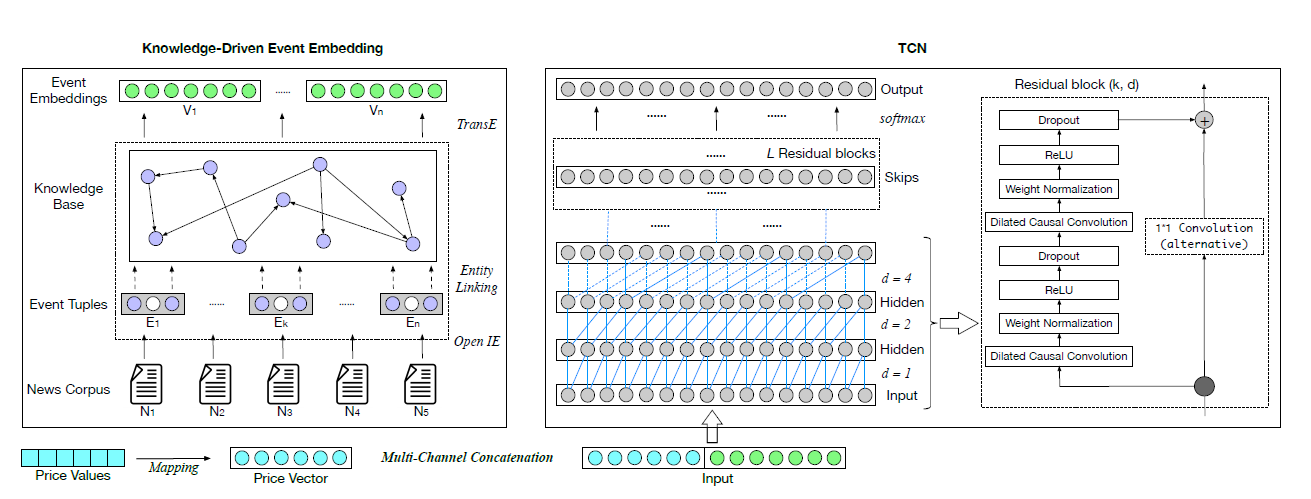
\includegraphics[width=\textwidth]{../Figures/ch_3_11_1.png}
\end{figure}

In the KDTCN architecture, the original model inputs are price values $\mathcal{X}$ , news corpus $\mathcal{N}$ , and knowledge graph $\mathcal{G}$. The price values are normalized and mapped into the price vector, denoted by
$$\mathcal{P}=\{p_0,p_1,\ldots,p_{T-1}\}$$
where each vector $p_t$ represents a real-time price vector on a stock trading day $t$ , and $T$  is the time span. Pieces of news are represented as event sets $\mathcal{E}$ , and event tuple is defined as $ e = (s,p, o)$, where $p$  is the action or predicate, $s$ is the actor or subject and $o$  is the object on which the action is performed. Then, each item in event tuples is linked to KG. Note that event items in this paper refer to the $s$, $p$ and $o$ ,  and  in the event tuple $(s, p, o)$ , and they also correspond to entities and relations in KG. They obtain event embeddings $\mathcal{V}$  by training both event tuples and KG triples. 
They propose $linking(e)$ and $linking(r)$ to define the entity and relation in an event tuple linked to KG, as well as $context\ (e)$ to define the immediate neighbors of linked entities in KG, denoted by
$$linking\left(e\right)={\{e}_i|e_i=s\vee o,\left(s,p,o\right)\in\mathcal{E}_t\land e_i\in\mathcal{G}\ \}$$ $$linking\left(r\right)=\{r_i|r_i=p\land\left(s,p,o\right)\in\mathcal{E}_t\land r_i\in\mathcal{G}\}$$
$$context\ (e)\ =\ \{e_i\ |\ (e_i\ ,\ r\ ,\ e)\ \in\ \mathcal{G}\ \vee\ (e,\ r\ ,\ e_i\ )\ \in\ \mathcal{G},\ e\ \in\ linking(e)\}$$

Then they parameterize event representations in different channels, denoted by $\mathcal{V}_l$ in the channel of KG linking,  $\mathcal{V}_c$ in the channel of KG context, and $\mathcal{V}_w$  in the channel of words.
$$\mathcal{V}_l=\left[\mathcal{V}_{e_l^s\ },\mathcal{V}_{r_l^p\ },\mathcal{V}_{e_l^o\ }\right]$$
$$\mathcal{V}_c=\left[\mathcal{V}_{e_c^s\ },\mathcal{V}_{r_c^p\ },\mathcal{V}_{e_c^o\ }\right]$$
$$\mathcal{V}_w=\left[\mathcal{V}_{e_w^s\ },\mathcal{V}_{r_w^p\ },\mathcal{V}_{e_w^o\ }\right]$$
where $e_l^s,e_l^o\in linking\left(e\right)$, and ${\ r}_l^p\in linking\left(r\right)$; $e_c^s,e_c^o\in context\left(e\right)$ , and $r_c^p\ \in\mathcal{G}$;  $\mathcal{V}_{e_w^s\ },\mathcal{V}_{r_w^p\ }$ and $\mathcal{V}_{e_w^o\ }$  are the word vectors of $s$, $p$ and $o$ respectively; $\mathcal{V}_\ast$ represents the embedding of $∗$. Then we concatenate $\mathcal{V}_l$, $\mathcal{V}_c $ ,  and $\mathcal{V}_w$   in multiple channels to get the final event embedding, denoted by
$$\mathcal{V}=F_e\left(\mathcal{E},\mathcal{G}\right)=\left[\mathcal{V}_l{\ \mathcal{V}}_c{\ \mathcal{V}}_w\right]$$
Finally, event embeddings, combined with price vectors are input into a TCN-based model for stock trend prediction and explanation particularly with abrupt changes.

\section{Other Derivatives(eg. Transformer)}

Several papers have studied using basic and modified attention mechanisms for time series data. LSTNet(Guokun Lai(2018)) is one of the papers that proposes using an LSTM + attention mechanism for multivariate forecasting time series. Temporal Pattern Attention for Multivariate Time Series Forecasting by Shun-Yao Shih et al. focused on applying attention specifically for multivariate data. This mechanism aimed to resolve issues including noisy variables in the multivariate time series and introduce a better method than a simple average. Neo Wu et al.(2020) employed Transformer-based machine learning models to forecast time series data. This approach works by leveraging self-attention mechanisms to learn complex patterns and dynamics from time-series data.